%%%%%%%%%%%%%%%%%%%%%%%%%%%%%%%%%%%%%%%%%
% Academic Title Page:
% LaTeX Template
% Version 2.0 (17/7/17)
%
% This TITLE PAGE template was downloaded from:
% http://www.LaTeXTemplates.com
%
% Original author:
% WikiBooks (LaTeX - Title Creation) with modifications by:
% Vel (vel@latextemplates.com)
%
% License:
% CC BY-NC-SA 3.0 (http://creativecommons.org/licenses/by-nc-sa/3.0/)
%
%%%%%%d%%%%%%%%%%%%%%%%%%%%%%%%%%%%%%%%%%%
% General Document Structure:
%
% The final research document should contain the following sections, typed in Times New Roman using 12-font size, 
% not more than 10 page with single line space:
%
% TITLE: What is the study about?
%
% PROPOSAL: A brief plan of intention, strategy and accomplishments (about ½-1 page).
%
% RATIONALE: Why is this study important? What is the purpose of the study? What do you want to achieve? (about ½-1 page).
%
% LITERATURE REVIEW: Mention any reference/example of similar/ related work/ article citation. Discuss briefly what has 
% been done in this problem/area of your interest (about 2-3 pages).
%
% DESIGN AND ANALYSIS: Objective of the study, data source, statistical model/tools/methodology, validity of the 
% assumptions if any, results of the study (graphs, tables will go here), results discussion, (interpretations/
% conclusions/inferences).
%
% CONCLUSION: Limitations of the study, Questions for further research.
%
% REFERENCES: A list of the references used in the article.
%
%%%%%%%%%%%%%%%%%%%%%%%%%%%%%%%%%%%%%%%%%

%----------------------------------------------------------------------------------------
%	PACKAGES AND OTHER DOCUMENT CONFIGURATIONS
%----------------------------------------------------------------------------------------

\documentclass[11pt, a4paper]{article}

\usepackage[margin=1in]{geometry} % Used to adjust margins, footers, etc.
\usepackage[utf8]{inputenc} % Required for inputting international characters
\usepackage[T1]{fontenc} % Output font encoding for international characters`
\usepackage{mathpazo} % Palatino font
\usepackage{indentfirst} % Will indent first paragraph after a section tag
\usepackage{amsmath} % Mathematics package
\usepackage[font=small,labelfont=bf]{caption} % Modify caption font
\usepackage[font=small,labelfont=bf]{subcaption} % Modify subcaption font
\usepackage{pdfpages} % Include exterior pdfs
\usepackage{float}
\restylefloat{table}
\usepackage{graphicx}
\graphicspath{ {./figures/} } % Setting path to fetch images 0
\usepackage{listings} % for reading in R

\begin{document}

%----------------------------------------------------------------------------------------
%	TITLE PAGE
%----------------------------------------------------------------------------------------

\begin{titlepage} % Suppresses displaying the page number on the title page and the subsequent page counts as page 1
	\newcommand{\HRule}{\rule{\linewidth}{0.5mm}} % Defines a new command for horizontal lines, change thickness here
	\center % Center everything on the page 
	
	%------------------------------------------------
	%	Headings
	%------------------------------------------------
	\textsc{\LARGE Eastern Michigan University}\\[1.5cm] % Main heading such as the name of your university/college
	\textsc{\Large Master's Research}\\[0.5cm] % Major heading such as course name
	\textsc{\large Department of Mathematics and Statistics}\\[0.5cm] % Minor heading such as course title

	%------------------------------------------------
	%	Title
	%------------------------------------------------
	
	\HRule\\[0.4cm]
	{\huge\bfseries Prostate Cancer: \\ [0.5cm] Multiple Logistic Regression}\\[0.4cm] % Title of your document
	\HRule\\[1.5cm]
	
	%------------------------------------------------
	%	Author(s)
	%------------------------------------------------
	
	\begin{minipage}{0.4\textwidth}
		\begin{flushleft}
			\large
			\textit{Author}\\
			\textsc{Jeffrey Osiwala} % Your name
		\end{flushleft}
	\end{minipage}
	~
	\begin{minipage}{0.4\textwidth}
		\begin{flushright}
			\large
			\textit{Supervisor}\\
			Prof. \textsc{Khairul Islam} % Supervisor's name
		\end{flushright}
	\end{minipage}
	
	% If you don't want a supervisor, uncomment the two lines below and comment the code above
	%{\large\textit{Author}}\\
	%John \textsc{Smith} % Your name
	
	%------------------------------------------------
	%	Date
	%------------------------------------------------
	
	%\vfill % Position the date 3/4 down the remaining page
	\vspace{2cm} December 3, 2020 % Date, change the \today to a set date if you want to be precise
	
	
	%------------------------------------------------
	%	Logo
	%------------------------------------------------
	
	%\vfill\vfill
	%\includegraphics[width=0.3\textwidth]{mompic}\\[1cm] % Include a department/university logo - this will require the graphicx package
	
	%----------------------------------------------------------------------------------------
	
	%\vfill % Push the date up 1/4 of the remaining page
	
\end{titlepage}


%----------------------------------------------------------------------------------------
%	DOCUMENT BODY
%----------------------------------------------------------------------------------------

%  Proposal
% proposal
%
% PROPOSAL: A brief plan of intention, strategy and accomplishments (about ½-1 page).
%
%----------------------------------------------------------------------------------------
%	PACKAGES AND OTHER DOCUMENT CONFIGURATIONS
%----------------------------------------------------------------------------------------
% none

\section{Proposal}
In a research study, a university medical center urology group was interested in the association between prostate-specific antigen (PSA) and a number of prognostic clinical measurements in men with advanced prostate cancer. Data were collected on 97 men who were about to undergo radical prostectomies. The data given has identifications numbers, and provides information on 8 other variables on each person. The 8 variables being: PSA Level, Cancer Volume, Weight, Age, Benign Prostatic Hyperplasia, Seminal Vesicle Invasion, Capsular Penetration, and Gleason Score. \par
With this available data set, I will carry out a complete logistic regression analysis by first creating a binary response variable Y, called high-grade-cancer, by letting Y=1 if Gleason Score equals 8, and Y=0 otherwise (i.e., if Gleason Score equals 6 or 7). Thus, the response of interest is high-grade-cancer (Y), and the pool of predictors include those previously mentioned. \par
My analysis will consider transformations of predictors, the inclusion of second-order predictors, analysis of residuals and influential observations, model selection, goodness of fit evaluation, and the development of an ROC curve. Additionally, I will discuss the determination of a prediction rule for determining whether the grade of disease is predicted to be high grade or not, model validation, and finally assess the strengths and weaknesses of my final model. \\


%  Rationale
% rationale
%
% RATIONALE: Why is this study important? What is the purpose of the study? What % do you want to achieve? (about ½-1 page).
%
%----------------------------------------------------------------------------------------
%	PACKAGES AND OTHER DOCUMENT CONFIGURATIONS
%----------------------------------------------------------------------------------------
% none


\section{Rationale}
Prostate Cancer is the most common cancer in American men. The American Cancer Society (ACS), a nationwide voluntary health organization, estimates 191,930 new cases of prostate cancer and over 33,000 deaths in year 2020 alone. Additionally, the typical cost of therapy to a prostate cancer patient is \$2,800/month after diagnosis (primarily from surgery and subsequently from office visits). A reliable and well understood testing/screening procedure needs to be in place to support early detection, and to minimize these current and unforgiving metrics. \par
Research suggests that prostate cancer typically begins as a pre-cancerous condition, and these conditions are sometimes found when a man has an invasive prostate biopsy (the removal of small pieces of the prostate to look for cancer.) If prostate cancer is found early as a result of \textit{screening}, it will probably be at an earlier and more treatable stage than if no screening were done. While this might seem like prostate cancer screening would always be a good thing, there are still issues surrounding screening procedures that make it unclear if the benefits outweigh the risks for most men. \par
For example, the popular PSA screening test is not 100\% accurate. This test can sometimes have abnormal results even when a man does not have cancer (false-positive result), or normal results when a man does have cancer (false-negative result). Consequently, false-positive results can lead to some men to get prostate biopsies (with risks of pain, infection, and bleeding) when they do not have cancer, and false-negative results can give men a false sense of security even though they may actually have cancer. \par
Another important issue is that even if screening does detect prostate cancer, doctors often cannot tell if the cancer is truly dangerous and needs to be treated. Prostate cancer can grow so slowly that it may never cause a man problems in his lifetime, and some men who seek screening may be diagnosed with a prostate cancer that they would have never known about otherwise. It would never have led to their death, or even cause any symptoms. Finding a "disease" like this that would never cause problems is known as \textbf{overdiagnosis}. \par
The problem with overdiagnosis in prostate cancer is that many of the men might still be treated with either surgery or radiation, either because the doctor cannot be sure how quickly the cancer might grow or spread, or the man is uncomfortable knowing he has cancer and is not receiving any treatment. The treatment of a cancer that would never have caused any problems is known as \textbf{overtreatment}, and the major downsides after surgery or radiation may include urinary, bowel, and/or sexual side effects that can seriously affect a man's quality of life. Thus, men and their doctors often struggle to decide if treatment is needed, or if the cancer can just be closely watched without being treated right away. Even when men are not treated right away, they still need regular blood PSA tests and prostate biopsies to determine if their need for treatment in the future. \par
For now, the ACS recommends that men thinking about getting tested for prostate cancer learn as much as they can so they can make informed decisions based on available information, discussions with their doctors, and their own views on the possible benefits, risks, and limits of prostate cancer screening. To combat and better navigate these difficulties, research needs to continue to grow the understanding of prostate cancer, and to build stronger predictive models which can improve the outlook of male lives, and also alleviate undo strain on the healthcare system.

%  Literature Review
% literature review
%
% LITERATURE REVIEW: Mention any reference/example of similar/ related work/ article citation. Discuss briefly what has 
% been done in this problem/area of your interest (about 2-3 pages).
%

\section{Literature Review}

\subsection{Predictor Variables}

\noindent An understanding of the predictor variables in this particular study can be seen as follows:

\begin{itemize}

	\item \textbf{PSA Level}: Serum prostate-specific antigen level [mg/ml]. \par
		-Prostate cancer can often be found early by testing for prostate-specific antigen (PSA) levels in a man's blood. However, the PSA test is not 100\% accurate. (CANCER.ORG) \\
		- The chance of having prostate cancer increases as PSA level increases, but there is no set cutoff point that can tell for sure if a man does or does not have prostate cancer.
		
	\item \textbf{Cancer Volume}: Estimate of prostate cancer volume [cc]. \par
		-Studies have suggested that inflammation of the prostate gland (prostatitis) may be linked to an increased risk of prostate cancer, but other studies have not found such a link. \\
		-Inflammation is often seen in samples of prostate tissue that also contain cancer. The link between the two it not clear, and it remains an active area of research. (CANCER.ORG)
		
	\item \textbf{Weight}: Prostate weight [gm]. \par
		-As related to cancer volume, studies have suggested that inflammation (and an increase is prostate weight) may be linked to an increased risk of prostate cancer. This relationship remains an active area of research. (CANCER.ORG)
		
	\item \textbf{Age}: Age of patient [years]. \par	
		-Prostate cancer is rare in men younger than 40, but the chance of having prostate cancer rises rapidly after age 50. About 6 in 10 cases of prostate cancer are found in men older than 65. (CANCER.ORG)
		
	\item \textbf{Benign Prostatic Hyperplasia}: Amount of benign prostatic hyperplasia [cm\textsuperscript{2}] \par
		-BPH is a term used to describe common, benign type of prostate enlargement caused by an increased number of normal prostate cells. This condition is more common as men get older and is not currently known to be linked to cancer. (CANCER.ORG)
		
	\item \textbf{Seminal Vesicle Invasion}: Presence of absence of seminal vesicle invasion: 1 if yes; 0 otherwise. \par
		-SVI is the presence of prostate cancer in the areolar connective tissue around the seminal vesicles and outside the prostate.(NCBI.NLM.NIG.GOV)
		
	\item \textbf{Capsular Penetration}: Degree of capsular penetration [cm]. \par
		-Cancer that has reached the outer wall of an organ (i.e. the prostate) is referred to as capsular penetration. Conversely, if cancer is strictly confined to the organ itself it is called organ-confined cancer. (PFC.ORG)
		
	\item \textbf{Gleason Score}: Pathologically determined grade of disease using total score of two patterns (summed scores were either 6, 7, or 8 with higher scores indicating worse prognosis). \par
		-A measure of how likely the cancer is to grow and spread quickly. This is typically determined by the results of the prostate biopsy, or surgery. (CANCER.ORG)
		
\end{itemize}

\subsection{Related Research}

Doctors are still studying if screening tests will lower the risk of death from prostate cancer. The most recent results from two large studies show conflicting evidence, and unfortunately did not offer clear answers. \par

The outcomes of both studies can be summarized as follows:

\begin{itemize}

\item Early results from a large study done in the United States found that annual screening with PSA and DRE (digital rectal exam - for a DRE, the doctor puts a gloved, lubricated finger into the rectum to feel the prostate gland) did detect more prostate cancers than in men not screened, but this screening did not lower the death rate from prostate cancer. However, questions have been raised about this study, because some men in the non-screening group actually were screened during the study, which may have affected the results.

\item A European study did find a lower risk of death from prostate cancer with PSA screening (done about every 4 years), but the researchers estimated that roughly 781 men would need to be screened (and 27 cancers detected) to prevent one death from prostate cancer.

\item Neither of these studies has shown that PSA screening helps men live longer overall (i.e. lowers the overall death rate).

\end{itemize}

Prostate cancer is often slow-growing, so the effects of screening in these studies might become more clear in coming years. Also, both of these studies are being continued to see if a longer follow-up will give clearer results.




%  Design and Analysis
% design and analysis
%
% DESIGN AND ANALYSIS: Objective of the study, data source, statistical model/tools/methodology, 
% validity of the assumptions if any, results of the study (graphs, tables will go here),
% results discussion, (interpretations/consclusions/inferences)
%
%----------------------------------------------------------------------------------------
%	PACKAGES AND OTHER DOCUMENT CONFIGURATIONS
%----------------------------------------------------------------------------------------
% none


\section{Design and Analysis}
To best model the dichotomous response variable, Y\textunderscore HighGradeCancer, in the Prostate Cancer case study, I will employ a multiple logistic regression model, where 1 indicates high grade cancer and 0 indicates not high grade cancer. \par
In statistics, if \(\pi = f(x)\) is a probability then \(\frac{\pi}{1-\pi}\) is the corresponding \textit{odds}, and the \textbf{logit} of the probability is the logarithm of the odds:
\begin{equation}
	logit(\pi) = log(\frac{\pi}{1-\pi})
\end{equation}

Now, simple logistic regression means assuming that \(\pi(x)\) is related to \(\beta_0 + \beta_1x\) (the \textit{logit response function}) by the logit function. By equating \(logit(\pi)\) to the logit response function, we understand that the logarithm of the odds is a linear function of the predictor. In particular, the slope parameter \(\beta_1\) is the change in the log odds associated with a one-unit increase in \textit{x}. This implies that the odds itself changes by the multiplicative factor \(e^{\beta_1}\) when \textit{x} increases by 1 unit.

\begin{equation}
	log(\frac{\pi}{1-\pi}) = \beta_0 + \beta_1x
\end{equation}

From here, straightforward algebra will then show the Simple Linear Regression Model:

\begin{equation}
	E[Y] = \pi(x) = \frac{e^{\beta_0 + \beta_1x}}{1+e^{\beta_0 + \beta_1x}}
\end{equation}

Next, this simple logistic regression model is easily extended to more than one predictor variable by inclusion of the following two vectors, in matrix notation:

\[
	\boldsymbol{\beta} = 
	\begin{bmatrix}
		\beta_0 \\ \beta_1 \\ \vdots \\ \beta_{p-1}
	\end{bmatrix} \quad
	\textbf{X} = 
	\begin{bmatrix}
		1 \\ X_1 \\ X_2 \\ \vdots \\ X_{p-1}
	\end{bmatrix} 
\]

With this notation, the simple logistic response function (Eqn. 3) extends to the multiple logistic response function as follows:

\begin{equation}
	E[Y] = \pi(\textbf{X}) = \frac{exp(\textbf{X}'\boldsymbol{\beta})}{1+exp(\textbf{X}'\boldsymbol{\beta})}
\end{equation}

Fitting the logistic regression to the sample data requires that the parameters \(\beta_0\), \(\beta_1\),\(\cdots\), \(\beta_{p-1}\) be estimated. This will be done using the maximum likelihood technique provided within the statistical packages of both \textbf{R} and \textit{Python}.

\subsection{Data Transformations and Standardization}
Variable transformation is an important technique to create robust models using logistic regression, and the appropriate transformations on continuous variables are necessary to optimize the model predictiveness. Because the predictors are linear in the log of the odds, it is often helpful to transform the continuous variables to create a more linear relationship. \par 
The raw data collected contained several predictors with high skewness values. A few concerning features were determined to be PSA Level (skewness = 4.39), Cancer Volume (skewness = 2.18), and Weight (skewness = 7.46). As a prepossessing step to reduce skewness, I elected to transform these continuous predictor variables using the log-transformation, and standardize \textit{all} the data on top of that. The standardization step was used to normalize the data, and did not affect any underlying distributions among the predictor variables. \par
The finalized data skewness is summarized directly below in Figure 1. 

\begin{figure}[H]
	\centering
	\includegraphics[scale=0.9]{final_skewness}
	\caption{Finalized Skewness Values of Transformed Predictor Variables.}
\end{figure}

Additionally, I've included the histogram of PSA Level vs. Cancer Volume in Figure 2 - a helpful visual for the two predictors which carried the most significance through much of my analysis, as we soon shall see. Notice how the distributions exhibit no notable skewness, are quite symmetrical, and are centered on zero.

\begin{figure}[H]
	\centering
	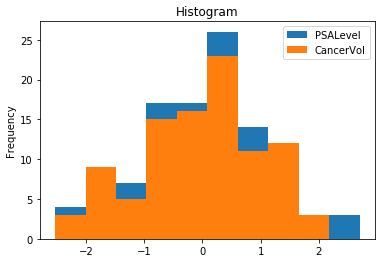
\includegraphics{psalevel_cancervol_skewness}
	\caption{Finalized PSALevel vs. CancerVol Histogram.}
\end{figure}

\subsection{Model Selection}
The data of 97 individual men in the Prostate Cancer sample was split at 80\% for train (model-building) and test (validation) sets. The training set is a random 76 observations and was used for fitting the model, and the remaining 21 cases were saved to serve as a validation data set. Figure 3 in columns 1-8 contains the variables, and shows a portion of the finalized and processed training data. \par

\begin{figure}[H]
	\centering
	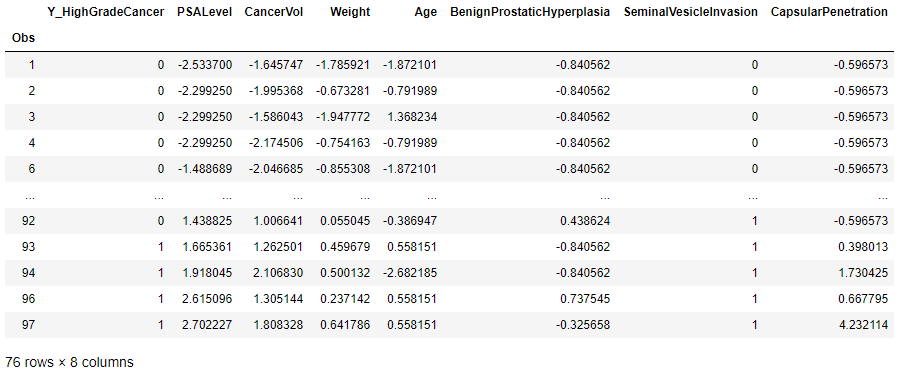
\includegraphics[scale=0.7]{train_data_python}
	\caption{Portion of Processed Model-Building Data Set - \textit{Python} Dataframe.}
\end{figure}

\pagebreak
\subsubsection{Best Subsets Procedure}
The procedure outlined here will help identify a group of subset models that give the best values of a specified criterion. This technique has been developed by time-saving algorithms which can find the most promising models, without having to evaluate all \(2^{p-1}\) candidates. The use of the best subset procedure is based on the \textit{AIC\textsubscript{p}} criteria, where promising models will yield a relatively small value. \par
The minimized \textit{AIC\textsubscript{p}} stepwise output given by \textbf{R} is provided in Figure 4 below.

\begin{figure}[H]
	\centering
	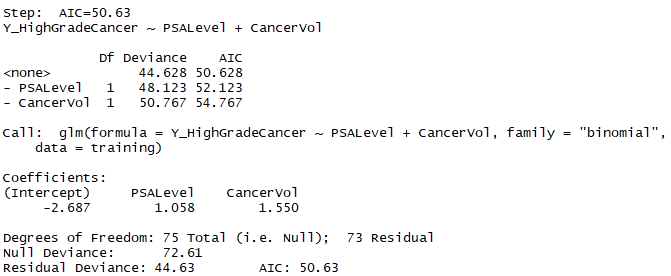
\includegraphics[scale=0.9]{best_subset}
	\caption{Full Linear Model  \textit{AIC\textsubscript{p}} Best Subset Results - \textbf{R} Output.}
\end{figure}

In this procedure, I instructed \textbf{R} to iterate "backwards" through all 7 predictor variables and it was determined \textit{AIC\textsubscript{p}} was minimized for \(p=3\). In particular, the results reveal that the best two-predictor model for this criteria is based on \textit{PSA Level} and \textit{Cancer Volume}. The \textit{AIC\textsubscript{p}} was minimized to 50.63, with a Null Deviance equal to 72.61 and Residual Deviance equal to 44.63. 

\subsubsection{Model Fitting}
A first-order multiple logistic regression model with two predictor variables was considered to be reasonable by \S4.2.1: 

\begin{equation}
\pi(\textbf{X}) = \frac{exp(\textbf{X}'\boldsymbol{\beta})}{1+exp(\textbf{X}'\boldsymbol{\beta})} = [1+exp(-\textbf{X}'\boldsymbol{\beta})]^{-1}
\end{equation}

where:

\begin{equation}
\textbf{X}'\boldsymbol{\beta} = \beta_0+\beta_1X_1+\beta_2X_2
\end{equation}

This model was then fit by the method of maximum likelihood to the data from the 76 random training cases. Results are summarized in the Figure 5 \textit{Python} output below. Provided in the output are the estimated coefficients, their standard errors, \textit{z}-scores, \textit{p}-values, and the accompanying 95\% confidence intervals. \par

\begin{figure}[H]
	\centering
	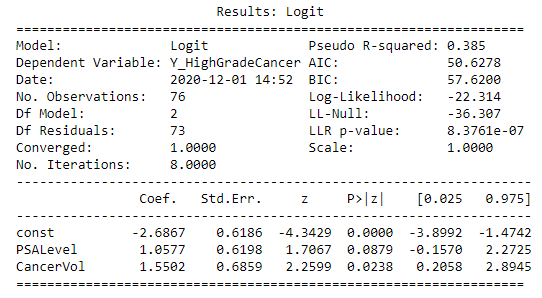
\includegraphics[scale=0.9]{model_fit_python}
	\caption{Maximum Likelihood Estimates of Logistic Regression Function - \textit{Python} Output.}
\end{figure}

Thus, the estimated logistic response function is:

\begin{equation}
\hat{\pi}=[ 1+ exp(-2.6867 + 1.0577X_1 + 1.5502X_2)]^{-1}
\end{equation}

\textbf{Note}: Although the PSALevel predictor is not of 5\% significance (\textit{p}-value=0.0879), I did find it necessary to maintain it within the model. When removed, the Residual Deviance score of 44.628 from Figure 4 rose to a value of 48.123. Therefore, I've deemed it significant, and a valuable and impactful variable to achieve high model accuracy, and have not removed it from this subset of predictors. \par
With the estimated logistic regression equation now developed, it is left to consider second-order options and make adjustments if required, analyze the residuals and influential observations, test goodness of fit, apply a prediction rule for new observations, and finally apply the final model to the validation data and evaluate the results.

\subsubsection{Geometric Interpretation}
When fitting a standard multiple logistic regression model with two predictors, the estimated regression shape is an S-shaped surface in three-dimensional space. Figure 6 displays a three-dimensional plot of the estimated logistic response function that depicts the relationship between the diagnosis of high grade prostate cancer (\textit{Y}, the binary outcome) and two continuous predictors, PSA Level (\textit{X}\textsubscript{1}) and Cancer Volume (\textit{X}\textsubscript{2}). \par
This surface increases in an approximately linear fashion with increasing values of PSA Level and Cancer Volume, but levels off and is nearly horizontal for very small and large values of these predictors.

\begin{figure}[H]
	\centering
	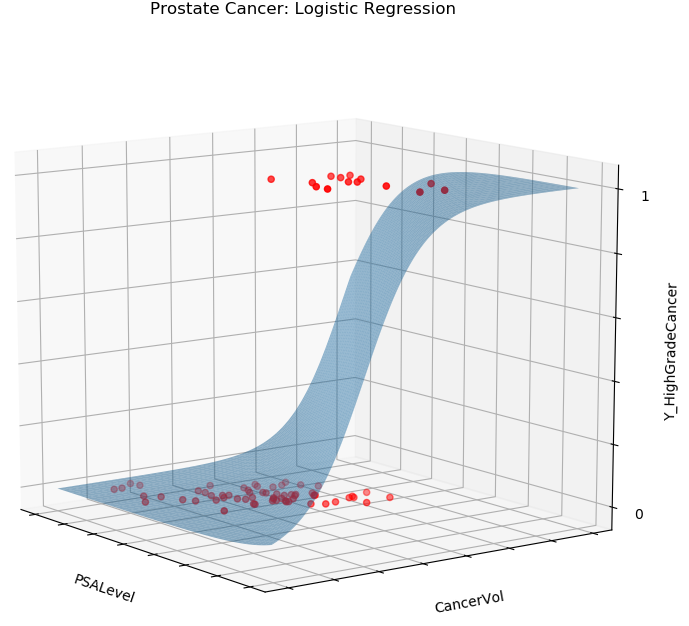
\includegraphics[scale=0.6]{3d_plot}
	\caption{Three-Dimensional Fitted Logistic Response Surface.}
\end{figure}

\subsubsection{Second-Order Predictors}
Occasionally, the first-order logistic model may not provide a sufficient fit to the data, and the inclusion of higher-order predictors may be considered. I'll conclude my model development stage by attempting to fit the Prostate Cancer data to a \textit{polynomial logistic} regression model of the second order, and analyze the results. \par 
For simplicity, a 2\textsuperscript{nd}-order polynomial model in \textit{two} predictors has a logit response function as:

\begin{equation}
logit(\pi) = \beta_0 + \beta_1x_1 + \beta_2x_2 + \beta_{11}x_1^2 + \beta_{22}x_2^2 + \beta_{12}x_1x_2
\end{equation}

\noindent and can be extended to more predictors by the inclusion of additional variables, their coefficients, and accompanying cross terms. Please recall, the Prostate Cancer data set considers 7 predictors. \par
In many situations the true regression function has one or more peaks or valleys, and in such cases a polynomial function can provide a satisfactory approximation. However, a polynomial fit was not successful here, as indicated by non-significant \textit{p}-values across all predictors, at 5\% significance (Figure 7). 

\begin{figure}[H]
	\centering
	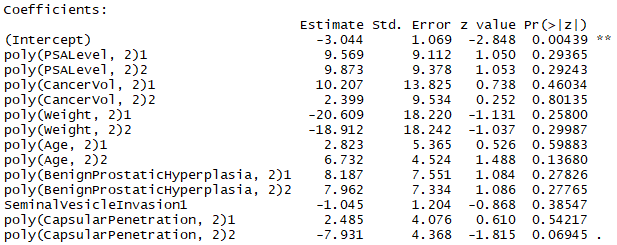
\includegraphics[scale=0.9]{poly_output}
	\caption{Logistic Regression Fit for Second-Order Model - \textbf{R} Output.}
\end{figure}

Additionally, my preliminary scatter plot analysis did not indicate any reason to believe a polynomial fit would be suitable in this study. For example, PSALevel was a major focus of this study and I've provided the scatter plot below in Figure 8. Additional scatter plots are provided in the Appendix, \S7.1.

\begin{figure}[H]
	\centering
	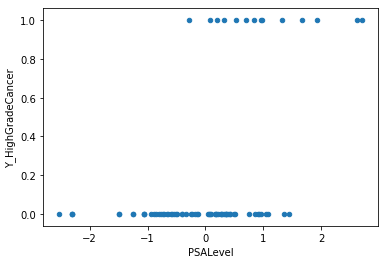
\includegraphics{psalevel_scatterplot}
	\caption{PSALevel vs Y\_HighGradeCancer Scatterplot - Train Data.}
\end{figure}

Without evidence to be concerned of successfully fitting a model with second-order predictors, I will move forward with my analysis of the previously developed multiple logistic linear regression model.


\subsection{Analysis of Residuals}
In this section I will discuss the analysis of residuals and the identification of any influential observations for logistic regression. Due to the nature of logistic regression, and the fact that non-constant variance is always present in this setting, I will focus only on the detection of model inadequacy.

\pagebreak
\subsubsection{Logistic Regression Residuals}
If the logistic regression model is correct, then \(E[Y_i]=\pi_i\) and it follows that:

\begin{equation}
E[Y_i-\hat{\pi}_i]=E[e_i]=0
\end{equation}

This suggests that if the model is correct, a lowess smooth of the plot of residuals against the linear predictor \(\hat{\pi}^{'}_i\) should result in approximately a horizontal line with zero intercept. Any significant departure from this suggests that the model may be inadequate. Shown in Figure 9 are the Pearson residuals plotted against the linear predictor, with the lowess smooth superimposed.

\begin{figure}[H]
	\centering
	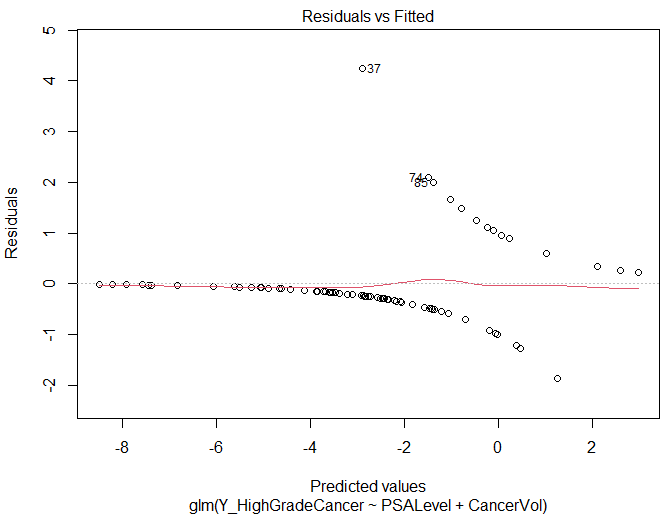
\includegraphics[scale=0.70]{residual_plot}
	\caption{Pearson Residual Plot with Lowess Smooth.}
\end{figure}

Looking at the plot, the lowess smooth adequately approximates a line having zero slope and zero intercept, and I conclude that no significant model inadequacy is apparent. 

\subsubsection{Influential Observations}
To aid in the identification of influential observations, I will use the \textbf{Cook's Distance} statistic, \(D_i\), which measures the standardized change in the linear predictor \(\hat{\pi}_i\) when the \textit{i}th case is deleted. Cook's distances are listed in the \textbf{R} Appendix \S7.2 for a portion of the Prostate Cancer testing data. \par
The plot of distances in Figure 10 identifies observation 90 as being the most outlying in the \textit{X} space, and therefore potentially influential - observations 37 and 91 also read relatively high values. Observation 90 was temporarily deleted and the logistic regression fit was obtained. The results were not particularly different from those obtained from the full test set, and the observation was retained. \textbf{Note}: I additionally and temporarily removed observations 37 and 91 and obtained a fit to the updated final model. The results were not particularly different, and those records were also retained. Thus, no changes to the model are yet necessary.

\begin{figure}[H]
	\centering
	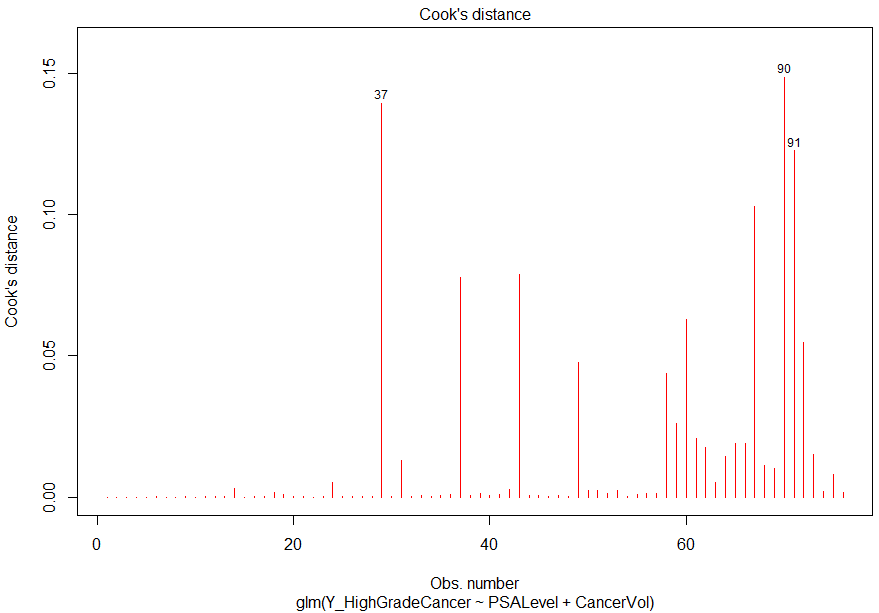
\includegraphics[scale=0.55]{cooks_distance}
	\caption{Index Plot of Cook's Distances.}
\end{figure}


\subsection{Goodness Of Fit Evaluation}
The appropriateness of the fitted logistic regression model needs to be examined before it is accepted for use. In particular, we need to examine whether the estimated response function for the data is monotonic and sigmoidal in shape, as are logistic response functions. Here I will employ the Hosmer-Lemeshow test, which is useful for unreplicated data sets, as is the Prostate Cancer data. The test can detect major departures from a logistic response function, and the alternatives of interest are as follows:

\begin{align}
\begin{split}
	H_0: E[Y]=  [1+exp(-\textbf{X}'\boldsymbol{\beta})]^{-1} \\
	H_1: E[Y] \neq  [1+exp(-\textbf{X}'\boldsymbol{\beta})]^{-1}
\end{split}
\end{align}

\subsubsection{Hosmer-Lemeshow}
The Hosmer-Lemeshow Goodness of Fit procedure consists of grouping that data into classes with similar fitted values \(\hat{\pi}_i\), with approximately the same number of cases in each class. Once the groups are formed, the Hosmer-Lemeshow goodness of fit statistic is calculated by using the Pearson chi-square test statistic of observed and expected frequencies. The test statistic is known to be well approximated by the chi-square distribution with \(c-2\) degrees of freedom.

\begin{equation}
	\chi^2 = \sum_{j=1}^{c} \sum_{k=0}^{1} \frac{(O_{jk}-E_{jk})^2}{E_{jk}}
\end{equation}

The output from \textbf{R} using 5 groups is shown in Figure 11 below.

\begin{figure}[H]
	\centering
	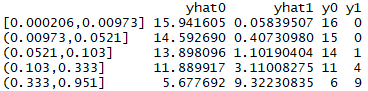
\includegraphics{gof_detail}
	% \caption{insert caption here}
	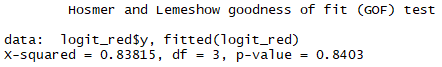
\includegraphics{gof_results}
	\caption{Hosmer-Lemshow Goodness of Fit Test for Logistic Regression Function.}
\end{figure}

Large values of the test statistic X\textsuperscript{2} indicate that the logistic response function is not appropriate. The decision rule for testing the alternatives (Eqn. 10) when controlling the level of significance at \(\alpha\) therefore is:

\begin{align}
\begin{split}
	\textrm{If X\textsuperscript{2}} \leq \chi^2(1-\alpha; c-p)\textrm{, conclude } H_0 \\
	\textrm{If X\textsuperscript{2}} > \chi^2(1-\alpha; c-p)\textrm{, conclude } H_1
\end{split}
\end{align}

Thus, for \(\alpha=0.05\) and \(c-2=5-2=3\), we require \(\chi^2(0.95; 3)=7.81\). Since \(X^2=0.838\leq7.81\), we conclude \textit{H}\textsubscript{0}, that the logistic response function is appropriate. The \textit{p}-value of the test is 0.8403.


\subsection{Development of ROC Curve}
Multiple logistic regression is often employed for making predictions for new observations.
The \textit{receiver operating characteristic} (ROC) \textit{curve} plots \(P(\hat{Y}=1 | Y=1)\) as a function of \(1-P(\hat{Y}=0 | Y=0)\) and is an effective way to graphically display prediction rule information, and possible cutoff points. \par
The "True Positive" \textit{y}-axis on an ROC curve is also known as \textit{sensitivity}, and the "False Positive" \textit{x}-axis is 1-\textit{specificity}. Figure 12 below exhibits the ROC curve for my model (Eqn. 7) for all possible cut points between 0 and 1.

\begin{figure}[H]
	\centering
	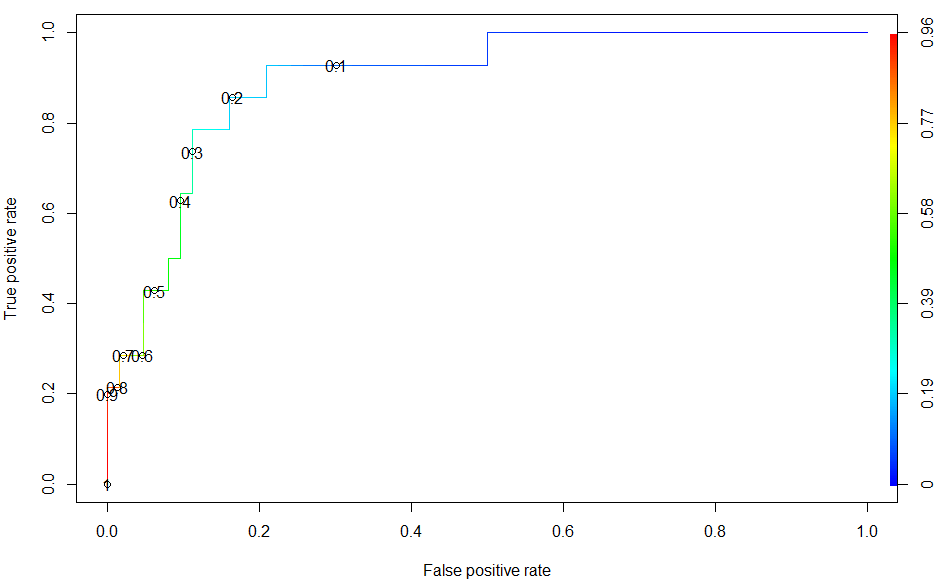
\includegraphics[scale=0.45]{roc}
	\caption{ROC Curve.}
\end{figure}

\subsubsection{Prediction Rule}
In the training data set (which represented a random 80\% of the 97 provided observations), there were 14 men who were observed as high grade cancer patients; hence the estimated proportion of persons who had high grade cancer is \(14/76=0.184\). This proportion can be used as the starting point in the search for the best cutoff in the prediction rule. \par
Thus, if \(\hat{\pi}_h\) represents a newly fitted observation, my first prediction rule investigated is:

\begin{equation}
	\textrm{Predict 1 if } \hat{\pi}_h \geq 0.184\textrm{; predict 0 if } \hat{\pi}_h < 0.184
\end{equation}

The Confusion Matrix of Table 1 below provides a summary of the number of correct and incorrect classifications based on the initial prediction rule (Eqn. 13). Of the 62 men without high grade cancer, 13 would be incorrectly predicted to have high grade cancer, or an error rate of 21.0\%. Furthermore, of the 14 persons with high grade cancer, 1 would be incorrectly predicted to not have high grade cancer, or 7.1\%. Altogether, \(13+1=14\) of the 76 predictions would be incorrect, so that the prediction error rate for the rule is \(14/76=0.184\) or 18.4\%. Coincidentally, the model exactly matches our training set proportions with the current prediction rule. \par

\begin{table}[H]
	\centering
	\begin{tabular}{ |c||c|c||c|  }
 	\hline
 	\multicolumn{4}{|c|}{Prediction Rule Eqn. 13} \\
 	\hline\hline
 	True Classification&\(\hat{Y}=0\)&\(\hat{Y}=1\)&Total\\
 	\hline
 	\(Y=0\)&49&13&62\\
 	\(Y=1\)&1&13&14\\
 	\hline\hline
 	Total&50&26&76\\
 	\hline
	\end{tabular}
 	\caption{Classification based on Logistic Response Function Eqn. 7 and Prediction Rule Eqn. 13.}
\end{table}

\pagebreak
With this baseline understood, it is straightforward to choose a stronger cutoff point in utilizing the ROC curve of Figure 12. As detailed above, the false-positive rate is not ideal at 21.0\% - there are too many cases where a man may opt for additional screening and treatment, even invasive actions, because he believes he has high grade prostate cancer. It will be wise to now reference the ROC curve to better choose a prediction cutoff, while also not significantly disturbing the false-negative accuracy for the worse. \par
Looking at Figure 12, a step occurs at 0.20 and I use this value for my new cutoff candidate. Thus, my updated prediction rule is stated as follows:

\begin{equation}
	\textrm{Predict 1 if } \hat{\pi}_h \geq 0.20\textrm{; predict 0 if } \hat{\pi}_h < 0.20
\end{equation}

and the effects of this change can be summarized by the Confusion Matrix in Table 2 below.

\begin{table}[H]
	\centering
	\begin{tabular}{ |c||c|c||c| }
 	\hline
 	\multicolumn{4}{|c|}{Prediction Rule Eqn. 14} \\
 	\hline\hline
 	True Classification&\(\hat{Y}=0\)&\(\hat{Y}=1\)&Total\\
 	\hline
 	\(Y=0\)&52&10&62\\
 	\(Y=1\)&2&12&14\\
 	\hline\hline
 	Total&54&226&76\\
 	\hline
	\end{tabular}
 	\caption{Classification based on Logistic Response Function Eqn. 7 and Prediction Rule Eqn. 14.}
\end{table}

Here, of the 62 men without high grade cancer, 10 are incorrectly predicted, or an error rate of 16.1\%. Continuing, of the 14 men with high grade cancer, 2 would be incorrectly predicted, or an error rate of 14.3\%. Altogether, updated prediction rule (Eqn. 14) now provides a total error rate of \(12/76=0.158\) or 15.8\%. Thus, the model accuracy has now increased with a significantly better false-positive rate, which is intended to reduce unnecessary financial stress across the healthcare economy.


\subsection{Model: Strengths and Weaknesses}
\subsubsection{Strengths}
-The two predictors which build the final logistic model are PSA Level and Cancer Volume, and they both are adequately correlated with the dependent (outcome) variable Y\_HighGradeCancer - their correlation values are 0.489 and 0.493, respectively. In fact, they are more correlated to the dependent variable than any other predictors of the data set. A consumable heat-map version of a correlation matrix is provided by Figure 13 below, with a color legend given in the upper-left corner.

\begin{figure}[H]
	\centering
	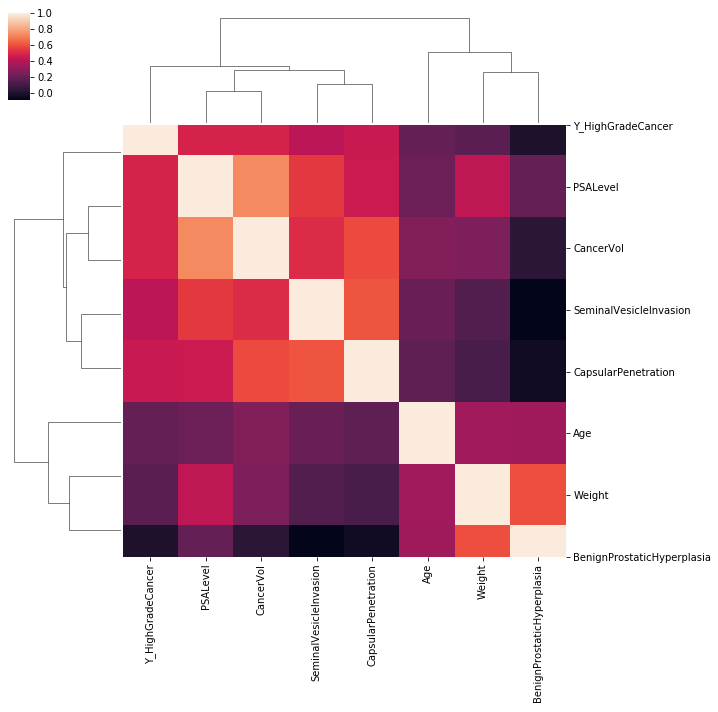
\includegraphics[scale=0.7]{corr_map}
	\caption{Correlation Heatmap - Train Data}
\end{figure}

-The final model has an excellent accuracy score of 84.2\% against training data. If this model also performs well in the validation step, then deploying such a model in use could possibly help non high grade cancer men be categorized as such, and thus not pursue unnecessary invasive testing and not inflate costs within the healthcare system. Also, by properly identifying those men who are high grade cancer patients, treatment and a plan can be devised sooner, as well as doing so by only use of PSA Level and Cancer Volume information, and not invasive testing. \\ 

\subsubsection{Weaknesses}
-An initial concern while building this model occurs at the level of the provided raw data, namely the existence of multicollinearity. Figure 14 below is the Correlation Matrix of the two final predictors which built the final logistic model: PSA Level and Cancer Volume.

\begin{figure}[H]
	\centering
	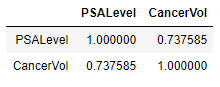
\includegraphics[scale=1.0]{corr_matrix}
	\caption{PSALevel vs. CancerVol Correlation Matrix - Train Data}
\end{figure}

\pagebreak
As shown, PSA Level and Cancer Volume have a mild correlation value of 0.738 in the full data set. One primary danger in designing models with multicollinearity is that small changes to the input data can lead to large changes in the model, which can further lead to over-fitting. Therefore, this logistic model may be considered mildly "noisy", sensitive, and not particularly robust. \\

-The Goodness of Fit Evaluation of \S4.4 deserves some concern regarding the Pearson chi-square test. As described previously, the Hosmer-Lemeshow procedure was utilized to determine a goodness of fit, and the test statistic is known to be well approximated by the chi-square distribution with \(c-2\) degrees of freedom (Eqn. 11). However, in view of the \textbf{R} output (Figure 11) with 5 groupings, the expected values (\textit{y\textsubscript{1}}) returned were: 0, 0, 1, 4, 9. Because many values are less than 5, and two of the expected values equal 0, the conditions for a chi-square test may be voided, and it may not be an appropriate test procedure here. At the very lest, the results of the Hosmer-Lemeshow test should be accepted carefully. \\

-The final model may produce high false-negative rates. In view of Figure 15-A we see that the first prediction cutoff of 0.184 produced 1 count of false-negatives (\(7.1\%\) error rate), and an overall model accuracy of \(81.6\%\). After ROC analysis the final prediction cutoff I've employed is 0.20. By Figure 15-B this rule produces 2 counts of false-negatives (\(14.3\%\) error rate), and an overall model accuracy of 84.2\%. Thus the overall model accuracy has improved 2.6 percentage points by correctly predicting more non high grade cancer cases, but has concurrently doubled the false-negative rate. Because correctly identifying high grade cancer patients may be considered most important, this arrangement may be a downfall of the final model.

\begin{figure}[H]
\centering
\begin{subfigure}{.5\textwidth}
  \centering
  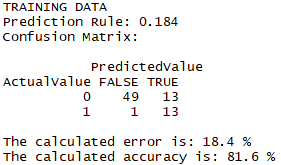
\includegraphics[width=.8\linewidth]{confusion_matrix_PR1}
  \caption{Confusion Matrix - 0.184 Cutoff Rule.}
  \label{fig:sub1}
\end{subfigure}%
\begin{subfigure}{.5\textwidth}
  \centering
  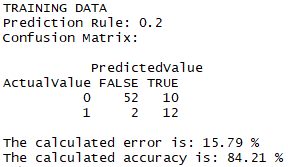
\includegraphics[width=.8\linewidth]{confusion_matrix_PR2}
  \caption{Confusion Matrix - 0.20 Cutoff Rule}
  \label{fig:sub2}
\end{subfigure}
\caption{Classification Based on Logistic Response Function (Eqn. 7) and Prediction Rules (Eqn. 13) and (Eqn. 14).}
\label{fig:test}
\end{figure}

%  Conclusion
% conclusion
%
% CONCLUSION: Limitations of the study, Questions for further research.
%
%----------------------------------------------------------------------------------------
%	PACKAGES AND OTHER DOCUMENT CONFIGURATIONS
%----------------------------------------------------------------------------------------
% none

\section{Conclusion}
\subsection{Model Validation}
The reliability of the chosen model, prediction rule, and prediction error rate from the training data is examined by now applying the prediction rule to the validation data set (i.e. the remaining 20\% of data). As I will show, the new prediction error rate is about the same as that for the model-building data set, and gives a reliable indication of the predictive ability of the fitted logistic regression model and the chosen prediction rule. If the new and unseen data had lead to a considerably higher prediction error rate, then the fitted logistic regression model and the chosen prediction rule would not predict new observations well. \par

\pagebreak
In my Prostate Cancer logistics model, the fitted logistic regression function (Eqn. 7) based on the model-building data set:

\[
\hat{\pi}=[ 1+ exp(-2.6867 + 1.0577X_1 + 1.5502X_2)]^{-1}
\]

was used to calculate estimated probabilities \(\hat{\pi}_h\) for the validation data set. The chosen prediction rule (Eqn. 14):

\[
	\textrm{Predict 1 if } \hat{\pi}_h \geq 0.20\textrm{; predict 0 if } \hat{\pi}_h < 0.20
\]

was then applied to these estimated probabilities. The percent prediction error rates are summarized in Figure 16 and Table 3 below:

\begin{figure}[H]
	\centering
	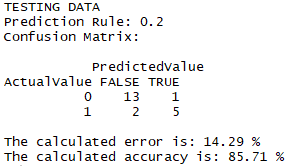
\includegraphics[scale=0.9]{confusion_matrix_final}
	\caption{Confusion Matrix - Validation Data}
\end{figure}

\begin{table}[H]
	\centering
	\begin{tabular}{ |c|c||c| }
 	\multicolumn{2}{c}{\underline{Disease Status}} \\
 	\hline
 	With High Grade Cancer&Without High Grade Cancer&Total\\
 	28.6\%&7.1\%&14.3\%\\
 	\hline
	\end{tabular}
 	\caption{Percent Prediction Error Rates - Validation Data}
\end{table}

Note that the total prediction error rate of 14.3\% is approximately equal to, or very similar to, the 15.8\% error rate based on the model-building data set. Therefore the latter is a reliable indicator of the predictive capability of the fitted logistic regression model and the chosen prediction rule. The accuracy is seen to be 85.7\%.

\subsection{Final Remarks}
The primary purpose of this study was to assess the strength of the association between each of the predictor variables with the response variable, the predictable nature of PSA Level, and the probability of a man having been diagnosed with high grade prostate cancer over low grade. We can now examine the odds ratios of the fitted model (Eqn. 7) to help address these questions. \par
The interpretation for multiple logistic regression is that the estimated odds ratio for the predictor variable \(X_k\) assumes that all other predictor variables are held constant. In view of the fitted model (Eqn. 7) the estimated coefficients are: \(\hat{\beta}_0 = -2.6867\), \(\hat{\beta}_1 = 1.0577\), and \(\hat{\beta}_2 = 1.5502\).
Therefore we can see, for instance, that the odds of a man being diagnosed with high grade prostate cancer increase by about 5.8\% for each additional score of PSA Level, for a given Cancer Volume. This means each unit increase of PSA Level increases the odds of said diagnosis by 5.8\%. Similarly, the odds of a man being diagnosed with high grade prostate cancer increase by  55.0\% for each unit increase in cancer volume. \par 
Thus, these calculated odds ratios suggest that Cancer Volume has a significantly larger association to the outcome (a diagnosis of high grade prostate cancer) than PSA Level. However, PSA Level proved more significant than all other predictors in my analysis of \S4.2, was used to achieve 85.7\% accuracy against validation data in \S5.1, and is both a cost-effective and noninvasive screening procedure for prostate cancer grade classification. \par
Lastly, because this study is observational by nature (all 97 selected men were predetermined to have been diagnosed with prostate cancer), we must be careful about the scope of inferences we draw. Since the data are observational, the result cannot be used as proof that high grade patients test with higher PSA Level; the possibility of confounding variables cannot be excluded. Furthermore, since the individuals were not said be be drawn at random from the population of men about to undergo radical prostectomies, inference to a broader population is not justified.


%  References
\pagebreak
% references
%
% REFERENCES: A list of the references used in the article.
%
%----------------------------------------------------------------------------------------
%	PACKAGES AND OTHER DOCUMENT CONFIGURATIONS
%----------------------------------------------------------------------------------------
%

\section{References}

Sample text. \\
Test.

%  Appendix
\pagebreak
% appendix
%
%----------------------------------------------------------------------------------------
%	PACKAGES AND OTHER DOCUMENT CONFIGURATIONS
%----------------------------------------------------------------------------------------
% none

%%% Python documentation %%%

% 1.0-jo-extract-prostate-data_cropped
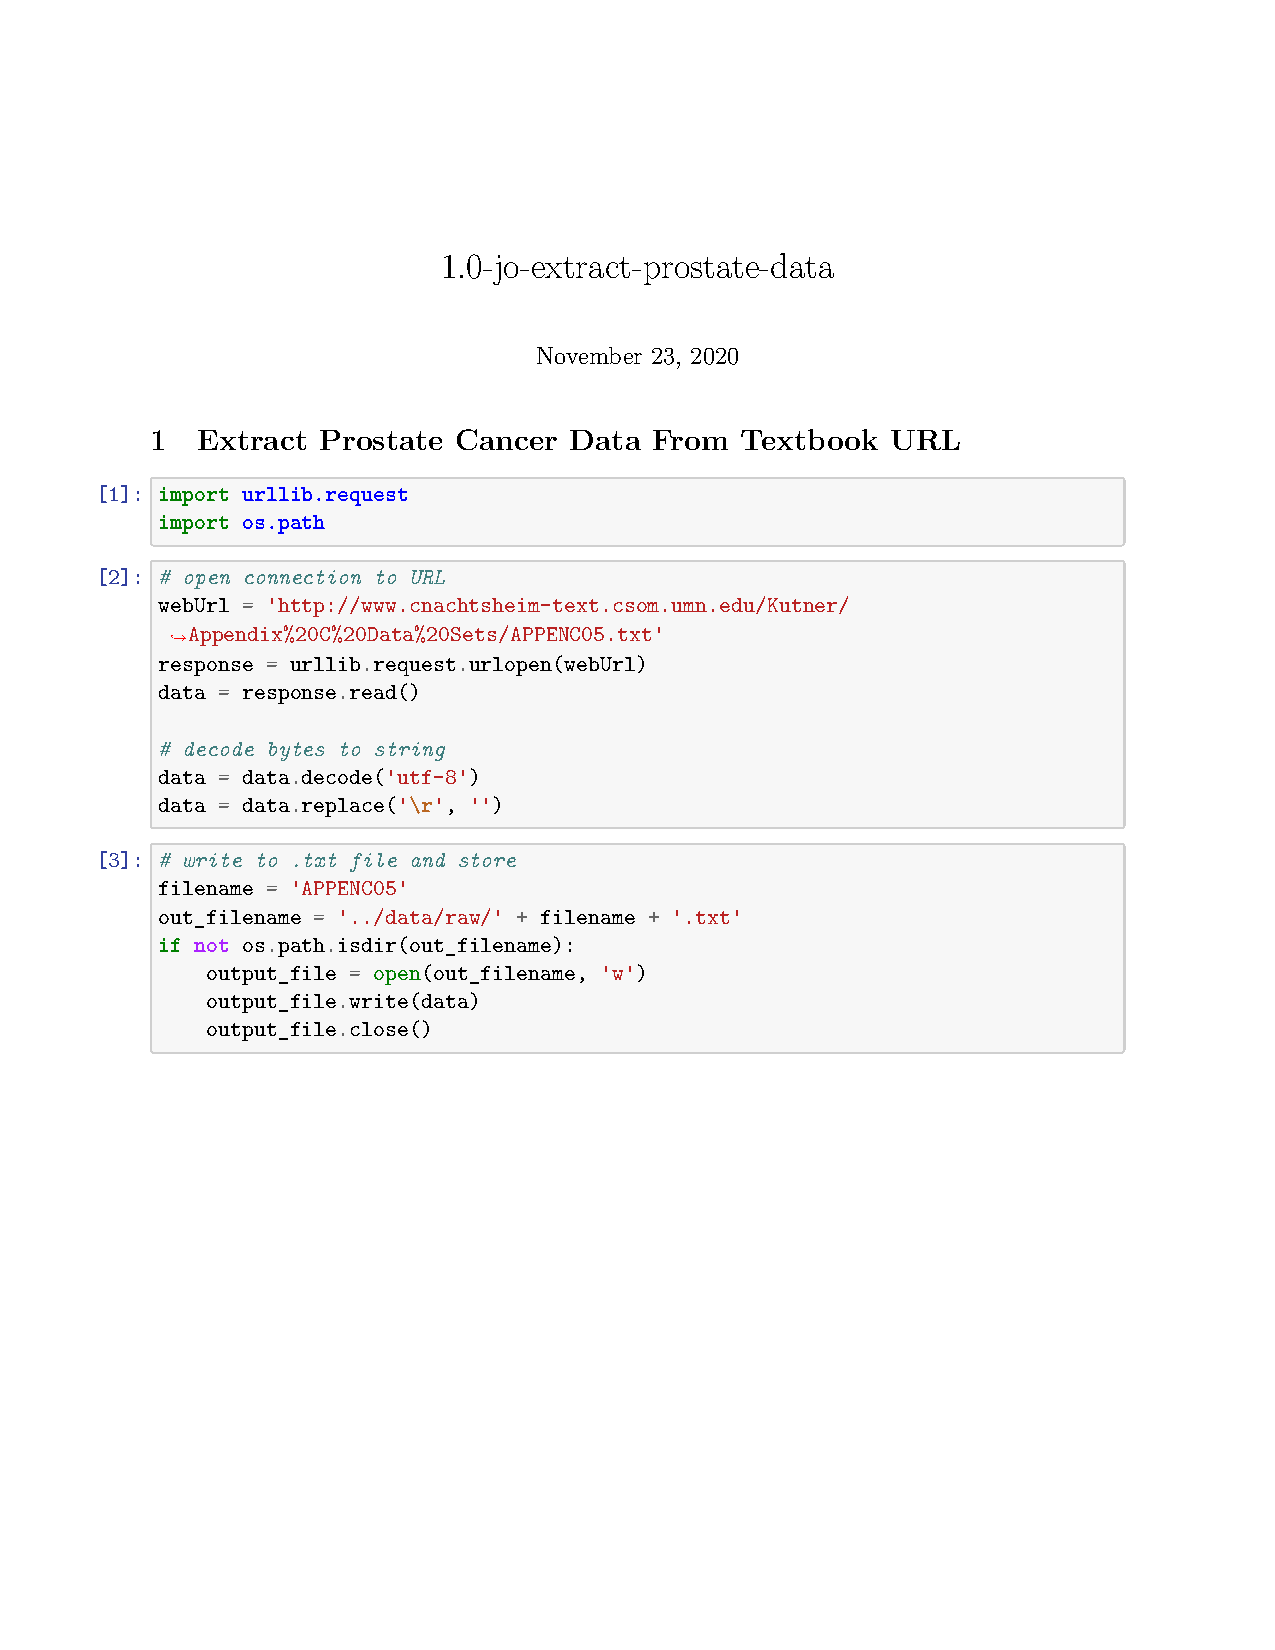
\includepdf[scale=0.95,pages=-,pagecommand=\section{Appendix}\subsection{Python}\thispagestyle{plain}]{../../docs/1.0-jo-extract-prostate-data_cropped}

% 2.0-jo-data-exploration_cropped
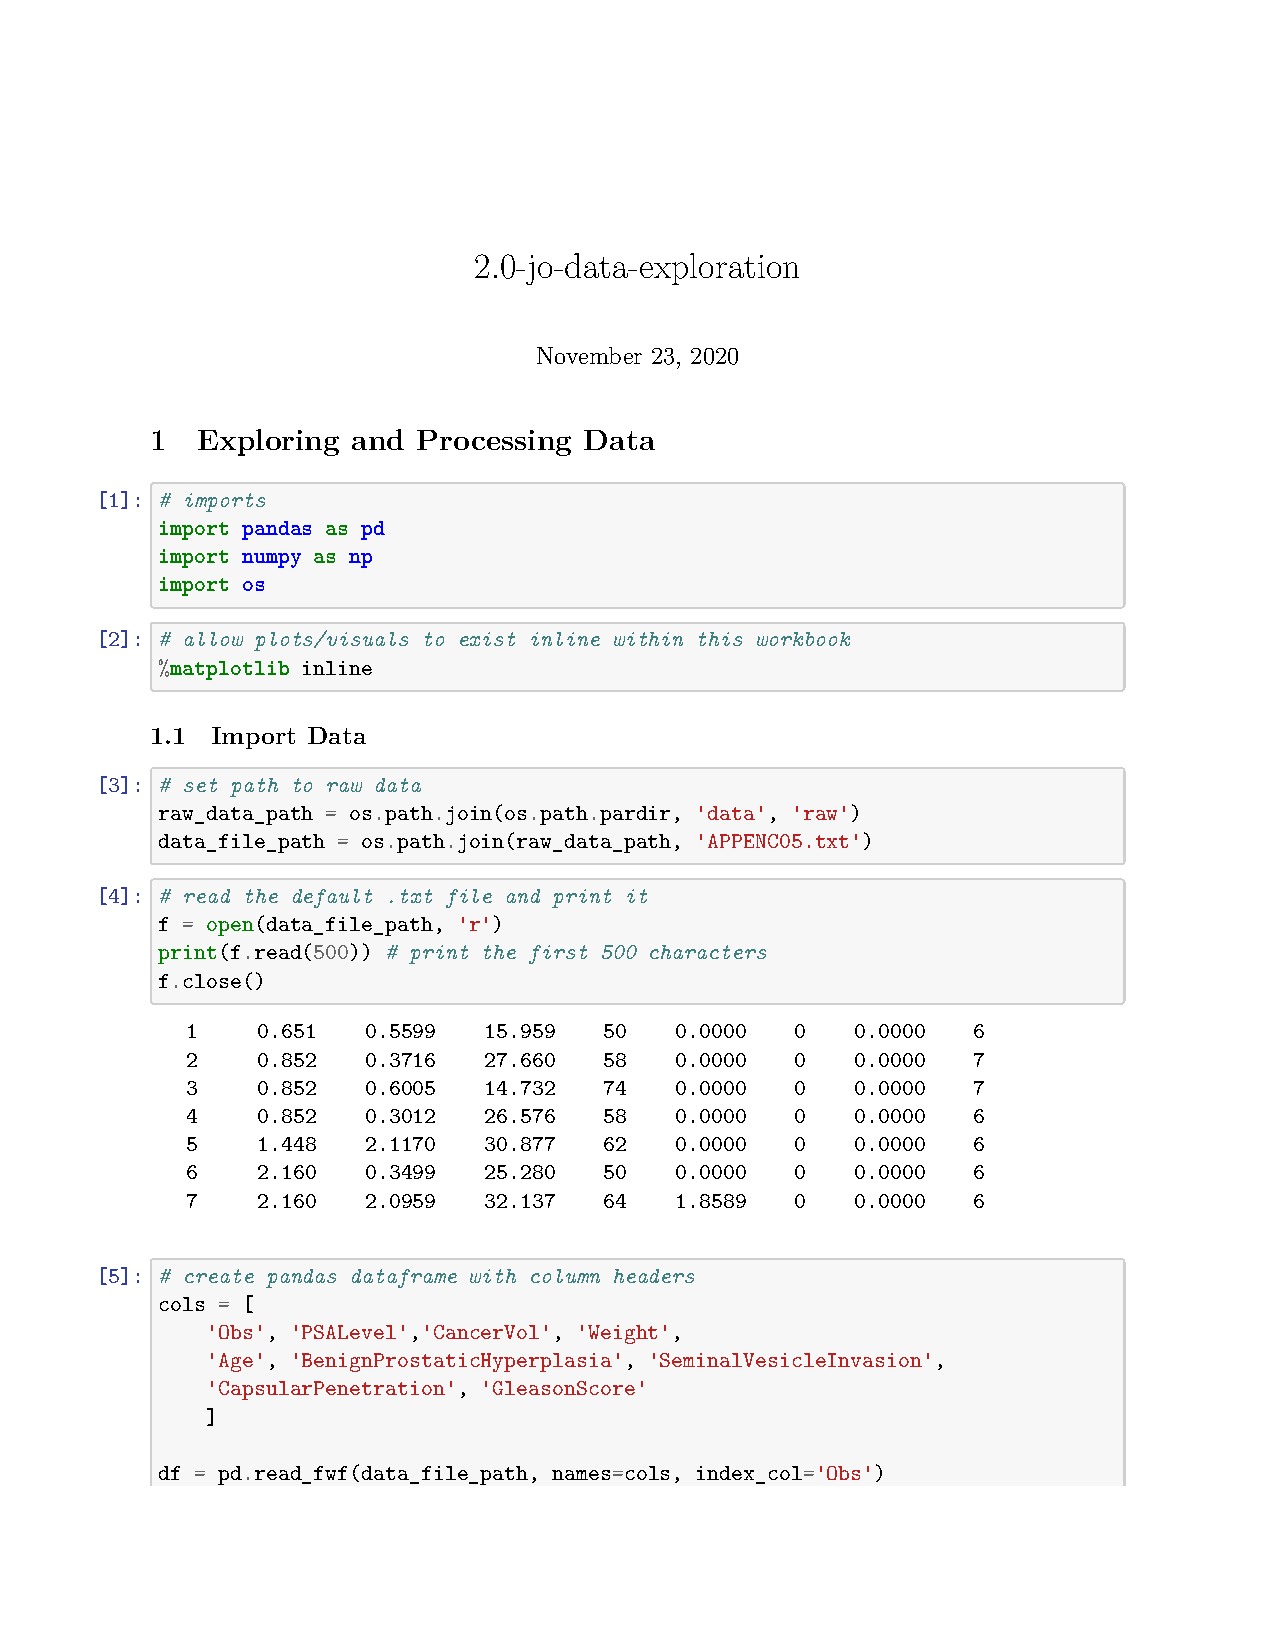
\includepdf[scale=0.95,pages=-,pagecommand={\thispagestyle{plain}}]{../../docs/2.0-jo-data-exploration_cropped}

% 3.0-jo-building-predictive-model_cropped
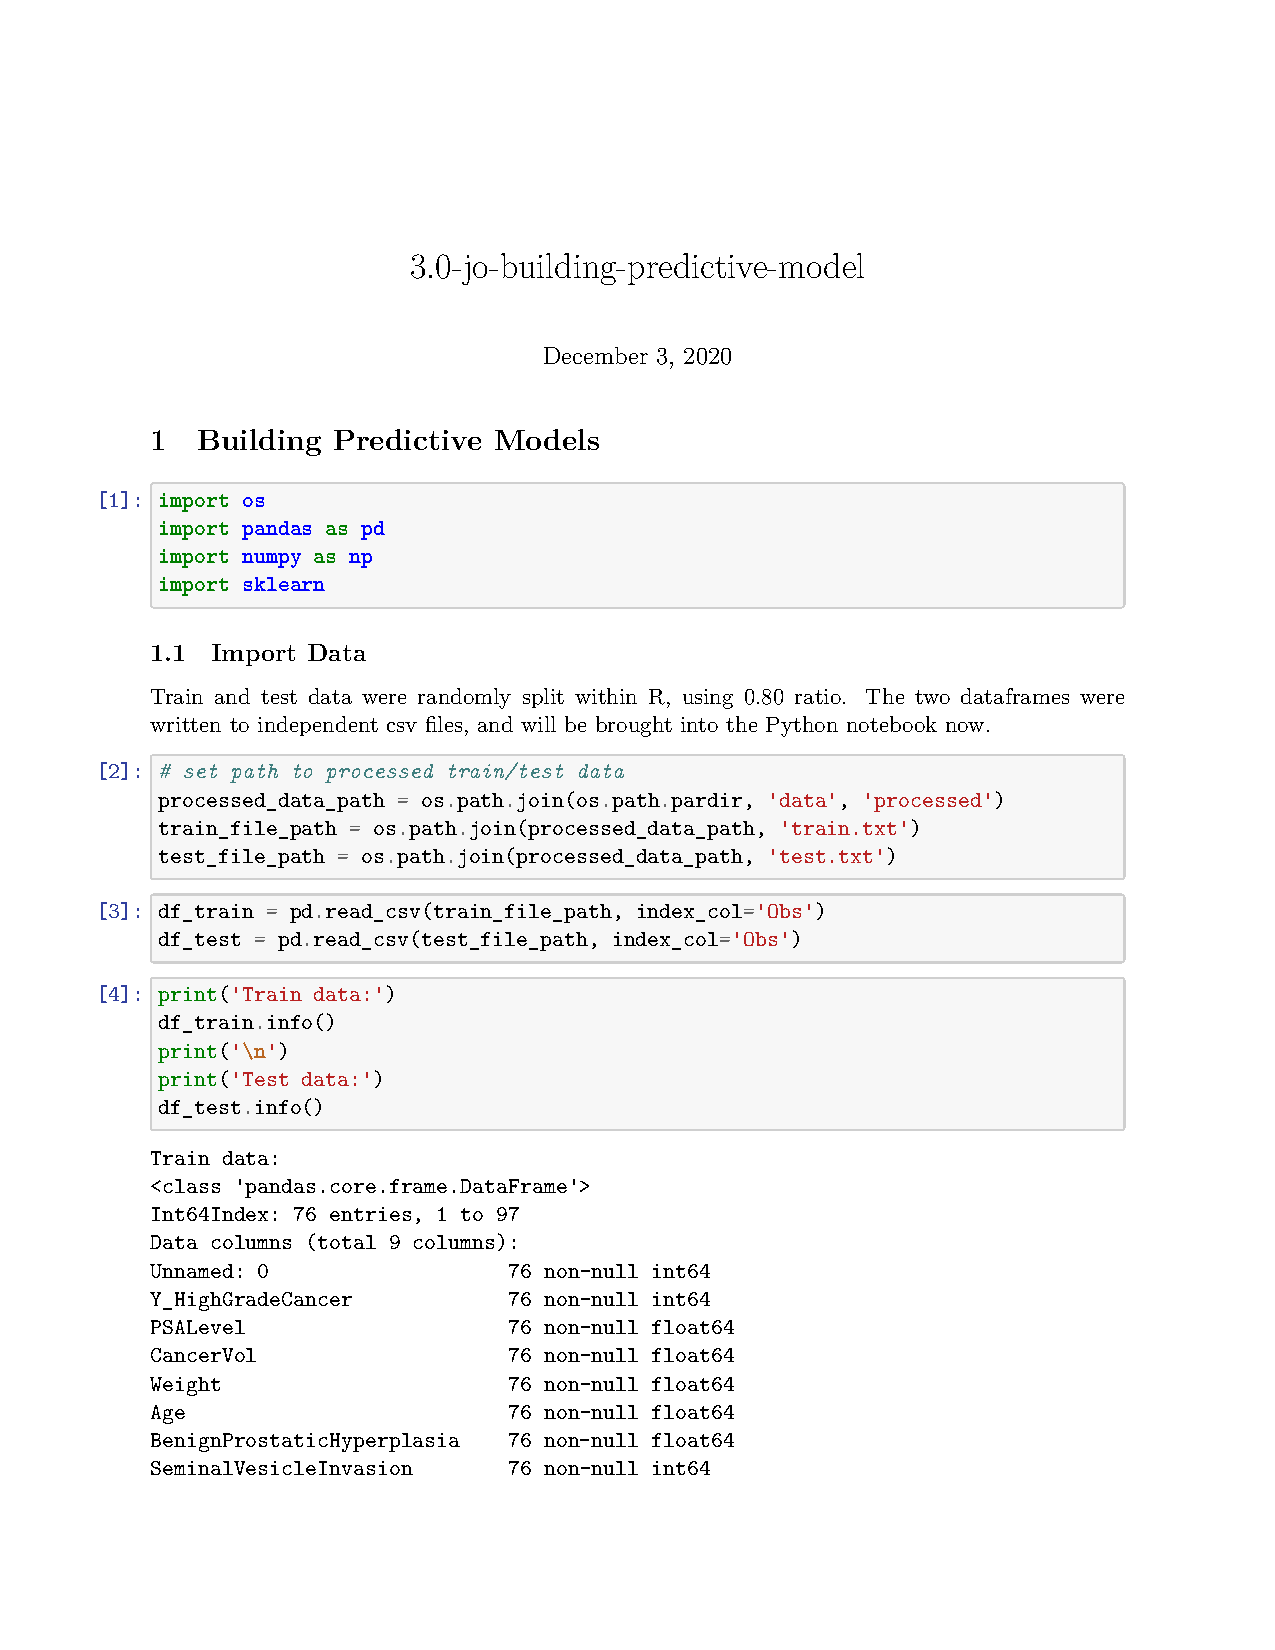
\includepdf[scale=0.95,pages=-,pagecommand={\thispagestyle{plain}}]{../../docs/3.0-jo-building-predictive-model_cropped}


%%% R documentation %%%

% Rscript_knitr
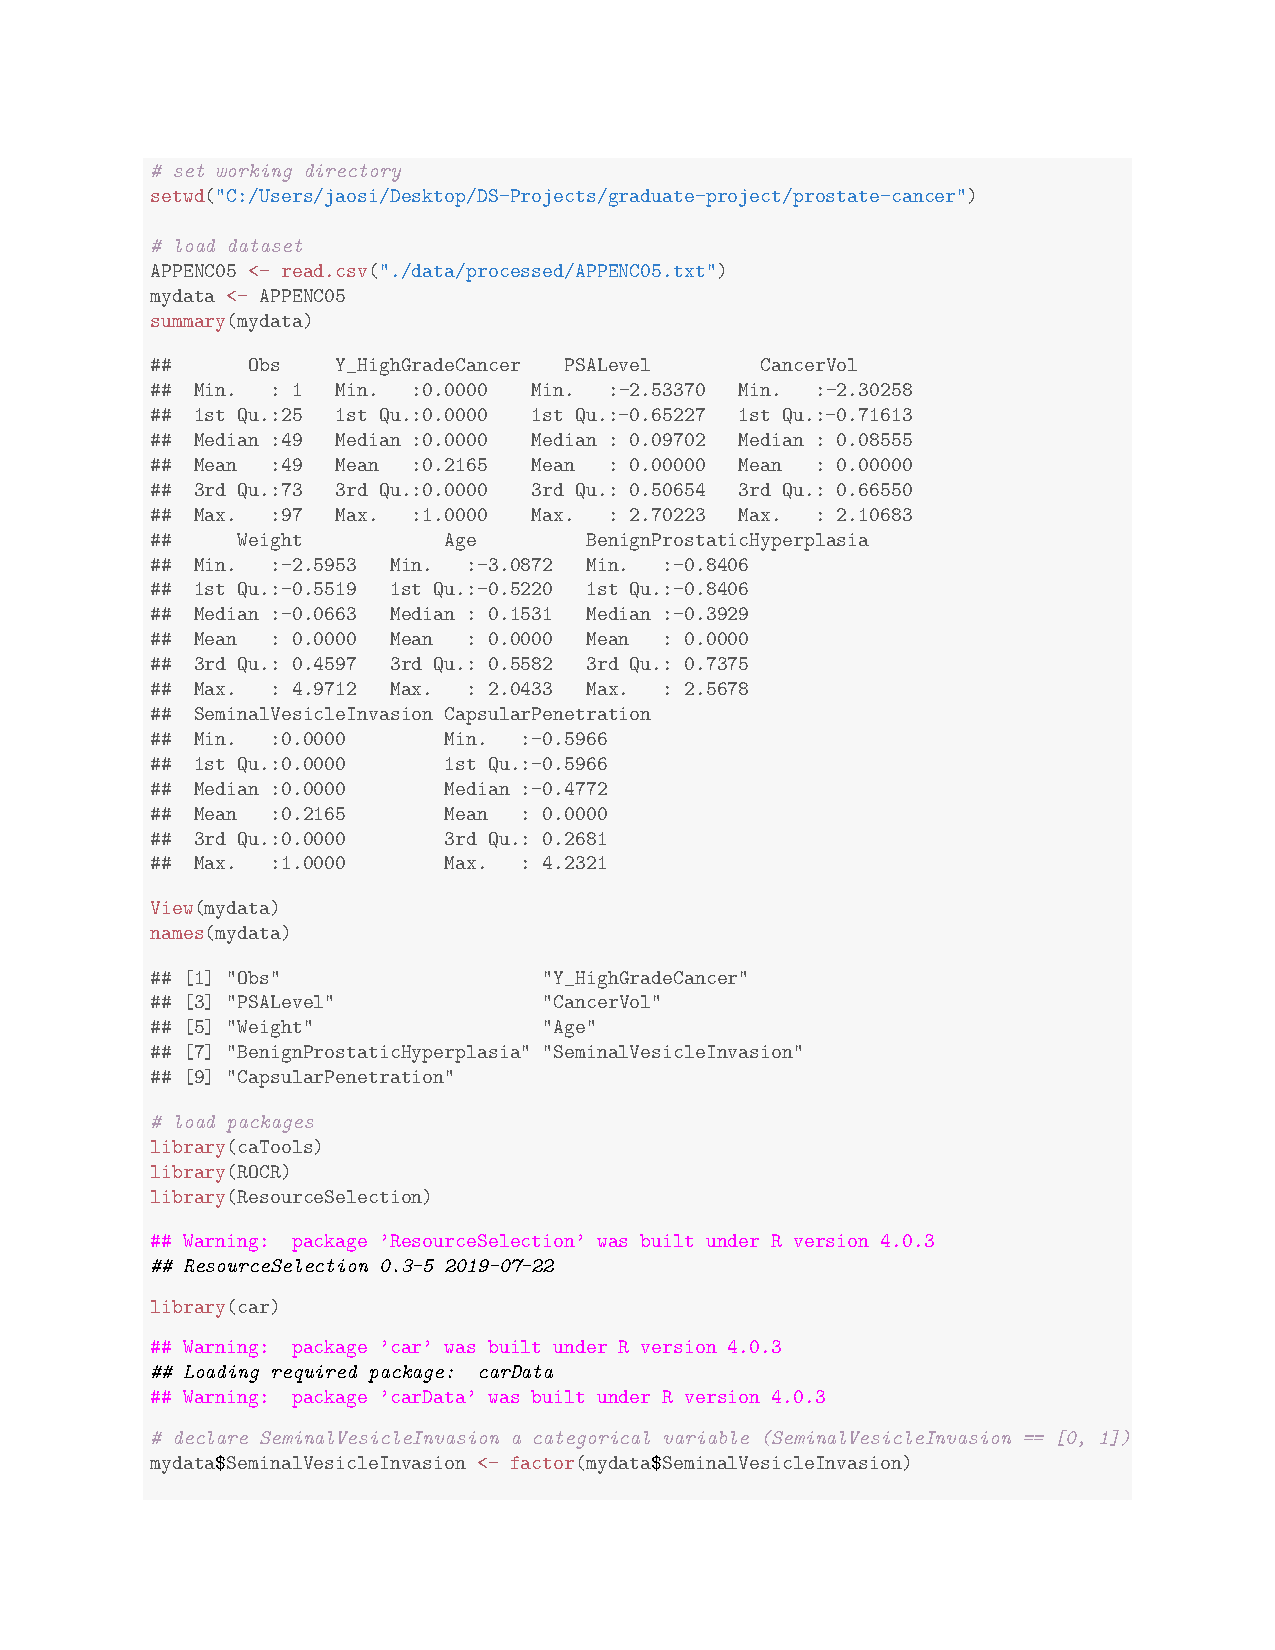
\includepdf[scale=1.0,pages=1,pagecommand=\subsection{R}\thispagestyle{plain}]{../../docs/Rscript_knitr_cropped}
\includepdf[scale=1.0,pages=2-17,pagecommand=\thispagestyle{plain}]{../../docs/Rscript_knitr_cropped}




\end{document}
